\section{Results}

First, we confirmed that France does not have enough
\gls{LWR} \gls{UNF} to transition into a fully \gls{SFR}
fleet. As shown in figure \ref{fig:only_france}, France
cannot meet the \gls{ASTRID} fuel demand without receiving
\gls{LWR} \gls{UNF} from other \gls{EU} nations. France
is able to fuel some of its \glspl{ASTRID} and breed more
plutonium, but cannot meet the fuel demand of 
all \glspl{ASTRID} with this aggressive deployment scheme.


\begin{figure}[htbp!]
	\begin{center}
		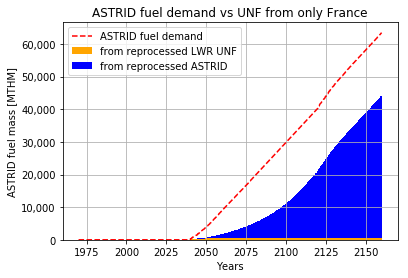
\includegraphics[scale=0.7]{./images/french-transition/france_only_compare.png}
	\end{center}
	\caption{\gls{ASTRID} fuel demand compared with fuel supply from only
			 France in the simulation. The lack of initial \gls{ASTRID} fuel
			 is caused by the lack of \gls{LWR} \gls{UNF} to reprocess. The
			 initial shortage then causes a decrease in plutonium bred by
			 \glspl{ASTRID}, thus a decrease in \gls{ASTRID} fuel supply.}
	\label{fig:only_france}
\end{figure}


\subsection{Nuclear Material Inventory}

Table \ref{tab:sim_result1} 
lists \gls{EU} material inventory in 2050.
The materials continue to accumulate after 2050, but the
\gls{UNF} France receives before 2050 is most impactful for the
feasibility of the transition. Note that table \ref{tab:sim_result1} 
distinguishes the
\gls{UOX} in the simulation either stored or reprocessed to create \gls{MOX}.


\begin{table}[h]
	\centering
        \caption{\gls{EU} nuclear material inventory in 2050.}
\begin{tabularx}{\textwidth}{XrX}
			\hline
                        \textbf{Category} & \textbf{Value} & Specifics \\
                                          & \textbf{[MTHM]} & \\ \hline
                        UOX Loaded  & 152,271 & UOX used in EU reactors 1970-2050\\ 
			MOX Loaded  & 6,463  & MOX used in French reactors 1970-2050\\
                        Available used UOX (EU)  & 85,111  & Used EU (minus France) 
                                UOX in storage for future ASTRID MOX 
                                production\\
                        Available used UOX (France) & 
                                12,582  & Used French UOX stored for 
                                future ASTRID MOX production. \\
                                Reprocessed UOX (France) & 51,511 & Used French UOX already reprocessed for the production of LWR MOX \\
			Tails  & 1,330,165  & (Tails generated) $-$ (Tails used for production of LWR MOX) \\ 
			Natural U Used  & 1,482,436  & \\ \hline
		\end{tabularx}
		
		\label{tab:sim_result1}
\end {table}
\FloatBarrier


Figures \ref{fig:eu_tail} and \ref{fig:eu_snf} show the 
accumulation of tails and used fuel over time in the \gls{EU}.
Tails accumulate as a by-product of uranium enrichment. 
Spent fuel is discharged from reactors every refueling period.
The entire core is discharged when the reactor decommissions.
A total of $1,330,165$ MTHM of tails and $85,111$ MTHM of
\gls{UNF} have accumulated by 2050.
Figure \ref{fig:eu_fuel} shows the amount of fuel used in the \gls{EU}. The 
tails mass accumulation rate is fairly steady, with peaks occurring when new 
reactors are deployed.
In figure \ref{fig:eu_snf}, the peaks are caused by reactor decommissioning which 
triggers all the batches in the final reactor core to be sent to the repository.

\begin{figure}[htbp!]
	\begin{center}
		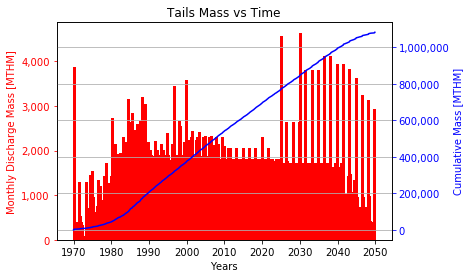
\includegraphics[scale=0.7]{./images/eu_future/tails.png}
	\end{center}
        \caption{Simulated accumulation of tails in the \gls{EU} is shown as a function of time.}
	\label{fig:eu_tail}
\end{figure}

\begin{figure}[htbp!]
	\begin{center}
		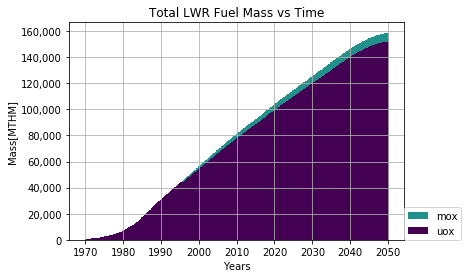
\includegraphics[scale=0.7]{./images/eu_future/total_fuel.png}
	\end{center}
\caption{Simulated total \gls{EU} fuel usage is shown as a function of time.}
	\label{fig:eu_fuel}
\end{figure}


\begin{figure}[htbp!]
	\begin{center}
			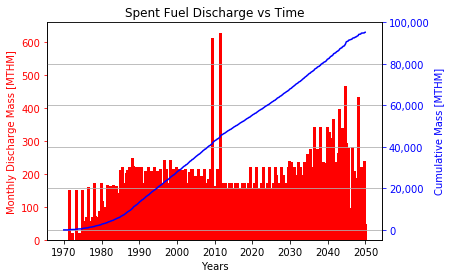
\includegraphics[scale=0.7]{./images/eu_future/snf_discharge.png}
	\end{center}
        \caption{Simulated \gls{EU} \gls{UNF} accumulation and discharge is 
shown as a function of time. The large peak near 2025 is due to the planned German
nuclear phase-out, in which all German reactors will have been decommissioned by 2022.}
	\label{fig:eu_snf}
\end{figure}


\subsection{French \gls{SFR} Deployment}
\FloatBarrier

Reprocessing the \gls{UNF} collected from all EU nations can provide
approximately 913 tons of plutonium. Table \ref{tab:pu} lists the 
isotope, mass fraction, and quantity of plutonium that can be obtained from the 
2050 \gls{UNF} inventory.  With the \gls{SFR} breeding ratio above one, France 
can transition into a fully \gls{SFR} fleet without extra construction of 
\glspl{LWR}. 

\begin{table}[h]
	\centering
	\caption{Plutonium in the \gls{UNF} inventory.}
	\begin{tabular}{lrr}
		\hline
		\textbf{Isotope} & \textbf{Mass Fraction in Used Fuel [\%]} & \textbf{Quantity [t]} \\ \hline
		Pu238 & 0.0111 & 9.76 \\ 
		Pu239 & 0.518 & 506.05 \\ 
		Pu240 & 0.232 & 226.64 \\ 
		Pu241 & 0.126 & 123.09 \\ 
		Pu242 & 0.0487 & 47.57 \\ \hline
		\textbf{Total} & \textbf{0.9358} & \textbf{913.14} \\ \hline
	\end{tabular}
	
	\label{tab:pu}
\end{table}

From Varaine et al. \cite{varaine_pre-conceptual_2012}, a French
ASTRID-type 600\gls{MWe} \gls{SFR} consumes $1.125$ metric tons of
plutonium a year, with an initial plutonium loading of $4.9$ metric tons.
 
Used \gls{MOX} from an ASTRID reactor is 23.95\% plutonium
in this simulation (see table \ref{tab:comp_fresh}), whereas fresh \gls{MOX} is 22\% plutonium.
The plutonium breeding ratio in this simulation is thus assumed to be
$\approx 1.08$.

Figure \ref{fig:fuel} shows \gls{MOX} loaded in the \glspl{SFR} per month.  The plot 
has peaks during a period of aggressive deployment of \glspl{SFR} followed by 
an equilibrium at 83 \gls{MTHM}. The peaks reoccur with the deployment of the 
second generation of \glspl{SFR}.  The spikes are due to initial fuel demand 
corresponding to these new deployments.  The initial cores loaded into new 
\glspl{SFR} rely on the \gls{MOX} created from legacy \gls{UNF}. Once the 
deployed \glspl{SFR} create enough extra plutonium, the legacy \gls{UNF} is no 
longer used. Notably, this switch from a less preferred fuel origin to a more 
preferred fuel origin is handled automatically within \Cyclus via user-defined preferences 
within its dynamic resource exchange algorithm \cite{gidden_methodology_2016}.


\begin{figure}[htbp!]
	\begin{center}
		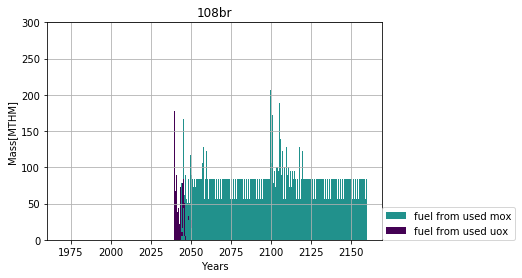
\includegraphics[width=1.0\textwidth]{./images/french-transition/where_fuel.png}
	\end{center}
	\caption{Fuel loaded into \glspl{SFR} was simulated in discrete 
        batches.}
	\label{fig:fuel}
\end{figure}

Figure \ref{fig:pu_no_cum} shows the separated plutonium discharge per 
month from the reprocessing plant. The plutonium outflux does not precisely 
follow the fuel demand because \Cyclus agents have material buffers that 
store commodity fuel for later usage. 
\gls{UNF} is stored for the initial loading of \glspl{SFR}.  Plutonium separated 
from legacy \gls{UNF} meets plutonium demands sufficiently to reduce the 
reprocessing demand for the first aggressive deployment of \glspl{SFR}.  
The plutonium from reprocessing legacy fuel is a flat rectangle because the 
reprocessing throughput was set to 183.2 $\frac{\gls{MTHM}}{month}$ to 
avoid reprocessing all the legacy in one timestep.
 

\begin{figure}[htbp!]
	\begin{center}
		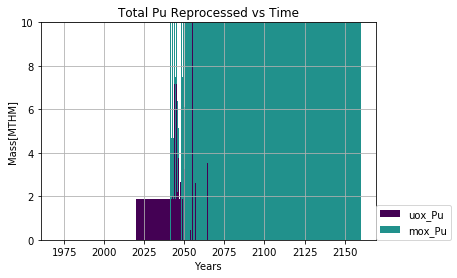
\includegraphics[scale=0.7]{./images/french-transition/pu.png}
	\end{center}
	\caption{The separated plutonium discharge from the reprocessing plant 
        in $\frac{\mbox{MTHM}}{\mbox{month}}$. The plutonium from \gls{LWR} \gls{UNF}
        is created after the demand is gone, due to material buffers in \Cyclus.}
	\label{fig:pu_no_cum}
\end{figure}

 Table \ref{tab:sfr_sim_result} lists French reprocessing and 
 \gls{ASTRID} fuel fabrication metrics.

\begin{table}[h]
	\centering
	\caption {In the French transition to \glspl{SFR},
				  the total legacy \gls{UNF} reprocessed is the 
                                  amount of \gls{UNF} France needs 
				  for a transition into a fully \gls{SFR} fleet. 
                          }
	\scalebox{0.86}{
		\begin{tabular}{llr}
			\hline
			\textbf{Category} & \textbf{Unit} & \textbf{Value}  \\ \hline
			Total \gls{ASTRID} MOX used & MTHM & 62,144  \\ 
			\textbf{Average UOX Reprocessing} & MTHM/month & \textbf{144.29} \\
			\textbf{Average Total Reprocessing} & MTHM/month & \textbf{61.3} \\
			\textbf{Average Fuel Fabrication} & MTHM/month & \textbf{36.9} \\
			Total \glspl{SFR} Deployed & & 214 \\ 
			Total Plutonium Reprocessed & MTHM & 13,671 \\ 
			Total \gls{ASTRID} fuel from UOX Waste & MTHM & 3,001  \\ 
			Total \gls{ASTRID} fuel from MOX Waste & MTHM  & 59,143 \\ 
			Total Tails used & MTHM & 48,472 \\ 
			\textbf{Total legacy UNF reprocessed} & MTHM & \textbf{55,553} \\ 
			Total Reprocessed Uranium Stockpile & MTHM & 194,186 \\ 
			Total Raffinate & MTHM & 12,123 \\ \hline
		\end{tabular}}
		
		\label{tab:sfr_sim_result}
\end {table}


These results demonstrate that despite the large amount of initial plutonium that has to be reprocessed
prior to \gls{ASTRID} deployment, the 20 years (2020-2040) of 
\gls{ASTRID} fuel preparation
allows a reasonable level of average
\gls{UOX} reprocessing capacity demand.